% This is samplepaper.tex, a sample chapter demonstrating the
% LLNCS macro package for Springer Computer Science proceedings;
% Version 2.20 of 2017/10/04
%
\documentclass[runningheads]{llncs2e/llncs}
%
\usepackage{graphicx}
\usepackage{xspace}
\usepackage[dvipsnames]{xcolor}
\usepackage{amsmath}
\usepackage{afterpage}  
\usepackage{figlatex,wrapfig}
\usepackage[dvipsnames]{xcolor}
\usepackage{listings,amssymb,mathtools}
\usepackage{mathrsfs}
\usepackage{array,multirow}
\usepackage{caption}
%\usepackage{textcomp}
\usepackage{algorithm}
\usepackage[noend]{algpseudocode}
\usepackage{framed,enumitem}

% for colours
\usepackage{xspace}
\usepackage[colorlinks]{hyperref}
\hypersetup{
	colorlinks = true,
	citecolor = {violet},
	linkcolor = {blue},
	urlcolor  = {blue}
}

% for arrow diagrams
\usepackage{amsmath}
\usepackage{amssymb}
\usepackage{smartdiagram}
\usepackage{tikz}
\usetikzlibrary{arrows,positioning}

%\usepackage[parfill]{parskip}

% for bib handline
%\usepackage[numbers]{natbib}
%\usepackage{url}

% implies and iff arrows
\renewcommand{\iff}{\xspace\Leftrightarrow\xspace}
\renewcommand{\implies}{\xspace\Rightarrow\xspace}
\newcommand{\onlyif}{\xspace\Leftarrow\xspace}

% commonly used abbreviations and expressions
\renewcommand{\th}{^{th}\xspace} % superscript th for numbers eg i^{th}
\newcommand{\definedas}{\triangleq\xspace}
\newcommand{\ie}{{\em i.e.}\xspace}
\newcommand{\st}{\ \mbox{s.t.}\ }
\newcommand{\viz}{\textit{viz}.\@\xspace}
\newcommand{\wrt}{\textit{wrt}\xspace}
\newcommand{\wkt}{we know that,\xspace}
\newcommand{\aka}{a.k.a\xspace}
\newcommand{\sota}{state-of-the-art\xspace}
\newcommand{\Sota}{State-of-the-art\xspace}

% common operators
\renewcommand{\^}{\xspace\wedge\xspace}
\renewcommand{\v}{\xspace\vee\xspace}
\newcommand{\xor}{\xspace\veebar\xspace}
\renewcommand{\|}{\ |\ }
\newcommand{\intersection}{\xspace\cap\xspace}
\newcommand{\union}{\xspace\cup\xspace}
\newcommand{\intersectioneq}{\xspace\cap=\xspace}
\newcommand{\unioneq}{\ {\cup}{=}\ }
\newcommand{\nin}{\not\in\xspace}

% highlighted hyperlinks
\newcommand{\hl}[1]{{\textcolor{darkgray}{\texttt{(#1)}}}\xspace} % hyperlink target
\newcommand{\hlref}[1]{\hyperlink{#1}{\textcolor{Sepia}{\small \texttt{(#1)}}}}
\newcommand{\tab}{\quad\quad}

%%%%%%%%%%%%%%%%%%%%%%%%% Document Specific %%%%%%%%%%%%%%%%%%%%%%

% names
\newcommand{\ourtechnique}{\textcolor{RubineRed}{\texttt{FenSyn}}\xspace}
\newcommand{\ourtool}{\ourtechnique{-}tool\xspace}
\newcommand{\cc}{\textit{C11}\xspace}

% sets and entitites
\newcommand{\program}{$P$\xspace} %input program
\newcommand{\programhat}{$\widehat{P}$\xspace} %transformed/fixed program
\newcommand{\fixed}[1]{\widehat{#1}\xspace}
\newcommand{\threads}{\mathcal{T}\xspace}
\newcommand{\states}{\Sigma\xspace}
\newcommand{\moset}{\mathcal{M}\xspace}
\newcommand{\actions}{\mathcal{A}\xspace}
\newcommand{\objects}{\mathcal{O}\xspace}
\newcommand{\s}[1]{s_{[#1]}\xspace} % state reached after exploring sequence #1
% events' sets aux
\newcommand{\wt}[1]{{\mathbb{W}#1}}
\newcommand{\md}[1]{{\mathbb{M}#1}}
\newcommand{\rd}[1]{{\mathbb{R}#1}}
\newcommand{\fn}[1]{{\mathbb{F}#1}}
% events' sets
\newcommand{\events}{\mathcal{E}\xspace}
\newcommand{\writes}{\events^\wt{}\xspace}
\newcommand{\reads}{\events^\rd{}\xspace}
\newcommand{\fences}{\events^\fn{}\xspace}
\newcommand{\ordevents}[1]{\events^{(#1)}\xspace}
\newcommand{\ordwrites}[1]{\events^\wt{(#1)}\xspace}
\newcommand{\ordreads}[1]{\events^\rd{(#1)}\xspace}
\newcommand{\ordfences}[1]{\events^\fn{(#1)}\xspace}


% memory orders
\newcommand{\mosc}{\texttt{seq\_cst}\xspace}
\newcommand{\moar}{\texttt{acq\_rel}\xspace}
\newcommand{\morel}{\texttt{release}\xspace}
\newcommand{\moacq}{\texttt{acquire}\xspace}
\newcommand{\mocon}{\texttt{consume}\xspace}
\newcommand{\morlx}{\texttt{relaxed}\xspace}

% operators
\newcommand{\molt}{{\sqsubset}\xspace}
\newcommand{\mole}{{\sqsubseteq}\xspace}
\newcommand{\mogt}{{\sqsupset}\xspace}
\newcommand{\moge}{{\sqsupseteq}\xspace}

% relations
\newcommand{\reln}[4]{#3 {\rightarrow^{#1}_{#2}} #4\xspace} % any relation specified as #1
\newcommand{\nreln}[4]{#3 \nrightarrow^{#1}_{#2} #4\xspace} % not of any relation specified as #1

% relation with events
\newcommand{\seqb}[3]{\reln{\textbf{\textcolor{CarnationPink}{sb}}}{#1}{#2}{#3}\xspace}
\newcommand{\rf}[3]{\reln{\textbf{\textcolor{PineGreen}{rf}}}{#1}{#2}{#3}\xspace} 
\newcommand{\dob}[3]{\reln{\textbf{\textcolor{Mulberry}{dob}}}{#1}{#2}{#3}\xspace}
\newcommand{\sw}[3]{\reln{\textbf{\textcolor{Magenta}{sw}}}{#1}{#2}{#3}\xspace}
\newcommand{\ithb}[3]{\reln{\textbf{\textcolor{NavyBlue}{ithb}}}{#1}{#2}{#3}\xspace}
\newcommand{\hb}[3]{\reln{\textbf{\textcolor{Cerulean}{hb}}}{#1}{#2}{#3}\xspace}
\newcommand{\nhb}[3]{\nreln{\textbf{\textcolor{Cerulean}{hb}}}{#1}{#2}{#3}\xspace}
\newcommand{\mo}[3]{\reln{\textbf{\textcolor{RedOrange}{mo}}}{#1}{#2}{#3}\xspace}
\newcommand{\nmo}[3]{\nreln{\textbf{\textcolor{RedOrange}{mo}}}{#1}{#2}{#3}\xspace}
\renewcommand{\to}[3]{\reln{\textbf{\textcolor{Brown}{to}}}{#1}{#2}{#3}\xspace}
\newcommand{\so}[3]{\reln{\textbf{\textcolor{Mahogany}{so}}}{#1}{#2}{#3}\xspace} %sc

% relation name without events
\newcommand{\setSB}{\seqb{\tau}{}{}\xspace}
\newcommand{\setRF}{\rf{\tau}{}{}\xspace}
\newcommand{\setSW}{\sw{\tau}{}{}\xspace}
\newcommand{\setDOB}{\dob{\tau}{}{}\xspace}
\newcommand{\setITHB}{\ithb{\tau}{}{}\xspace}
\newcommand{\setHB}{\hb{\tau}{}{}\xspace}
\newcommand{\setMO}{\mo{\tau}{}{}\xspace}
\newcommand{\setTO}{\to{\tau}{}{}\xspace}
\newcommand{\setSO}{\so{\tau}{}{}\xspace}
\newcommand{\nsetHB}{\nhb{\tau}{}{}\xspace}
\newcommand{\nsetMO}{\nmo{\tau}{}{}\xspace}

% relation label 
\newcommand{\lsb}{\textbf{\textcolor{CarnationPink}{sb}}\xspace}
\newcommand{\lrf}{\textbf{\textcolor{PineGreen}{rf}}\xspace} 
\newcommand{\ldob}{\textbf{\textcolor{Mulberry}{dob}}\xspace}
\newcommand{\lsw}{\textbf{\textcolor{Magenta}{sw}}\xspace}
\newcommand{\lithb}{\textbf{\textcolor{NavyBlue}{ithb}}\xspace}
\newcommand{\lhb}{\textbf{\textcolor{Cerulean}{hb}}\xspace}
\newcommand{\lmo}{\textbf{\textcolor{RedOrange}{mo}}\xspace}
\newcommand{\lto}{\textbf{\textcolor{Brown}{to}}\xspace}
\newcommand{\lso}{\textbf{\textcolor{Mahogany}{so}}\xspace}

\newcommand{\var}[1]{\color{OliveGreen}\texttt{#1}\color{black}\xspace}
\newcommand{\fun}[2]{\color{Sepia}\texttt{#1(\color{Gray}\textit{#2}\color{Sepia})}\color{black}\xspace}
\newcommand{\class}[1]{\color{DarkOrchid}\texttt{#1}\color{black}\xspace}

% memory orders
\newcommand{\na}{\texttt{na}\xspace}
\newcommand{\rlx}{\texttt{rlx}\xspace}
\newcommand{\rel}{\texttt{rel}\xspace}
\newcommand{\acq}{\texttt{acq}\xspace}
\newcommand{\acqrel}{\texttt{acq-rel}\xspace}
\renewcommand{\sc}{\texttt{sc}\xspace}

%snj: Have to use the ones in format
%\newtheorem{theorem}{Theorem}[section]
%\newtheorem{corollary}{Corollary}[theorem]
%\newtheorem{lemma}[theorem]{Lemma}

\newcommand{\ishComment}[1]{\textit{\color{red}\tiny{#1}}}
\newcommand{\divComment}[1]{\textit{\color{ForestGreen}{#1}}}
\newcommand{\snj}[1]{\textcolor{Mahogany}{[snj]: #1}}

% Used for displaying a sample figure. If possible, figure files should
% be included in EPS format.
%
% If you use the hyperref package, please uncomment the following line
% to display URLs in blue roman font according to Springer's eBook style:
% \renewcommand\UrlFont{\color{blue}\rmfamily}

\begin{document}
%
\title{Optimal Fence Synthesis for C/C++11}
%
%\titlerunning{Abbreviated paper title}
% If the paper title is too long for the running head, you can set
% an abbreviated paper title here
%
\author{First Author\inst{1}\orcidID{0000-1111-2222-3333} \and
Second Author\inst{2,3}\orcidID{1111-2222-3333-4444} \and
Third Author\inst{3}\orcidID{2222--3333-4444-5555}}
%
\authorrunning{F. Author et al.}
% First names are abbreviated in the running head.
% If there are more than two authors, 'et al.' is used.
%
\institute{Princeton University, Princeton NJ 08544, USA \and
Springer Heidelberg, Tiergartenstr. 17, 69121 Heidelberg, Germany
\email{lncs@springer.com}\\
\url{http://www.springer.com/gp/computer-science/lncs} \and
ABC Institute, Rupert-Karls-University Heidelberg, Heidelberg, Germany\\
\email{\{abc,lncs\}@uni-heidelberg.de}}
%
\maketitle              % typeset the header of the contribution
%
\begin{abstract}
The abstract should briefly summarize the contents of the paper in
150--250 words.

\keywords{\cc  \and Fence Synthesis \and Another keyword.}
\end{abstract}
%
%
%
\section{Introduction} \label{sec:intro}

\section{Preliminaries} \label{sec:preliminaries}
Consider a\deleted{n acyclic} multi-threaded \cc
program \added{$P$ $:=$ $\parallel_{i\in \text{\tt TID}} P_i$, 
where $\text{\tt TID}= \{1,\ldots,n\}$ is the set of thread ids}. 
\deleted{The} \added{Each} thread \deleted {of the program}
\added{$P_i$ is a loop-free program, which}
performs a sequence of memory access operations on a set of shared
memory objects and \cc memory fences.  The memory access operations
can be atomic or non-atomic in nature.
%
An instance of a thread operation in an execution is called an {\em
event}.  Events of a thread $t$ are uniquely indexed with an id.
%
\begin{definition}[Event]\newline
An event $i$ of thread $t$ is represented by a tuple $\langle i, t, act, obj,$ $ ord, inst \rangle$ where:
\begin{itemize}[label=inst,align=left,leftmargin=*]
\item [$act$] represents the event action $\in \{ \text{\tt read}, \text{\tt write}, \text{\tt rmw}, \text{\tt fence} \} $,
\item [$obj$] is the set of memory objects accessed,
\item [$ord$] records the \cc memory order associated with the event, and
\item [$inst$] is the corresponding program instruction.
\end{itemize}
\end{definition}
The $act$ {\tt rmw} represents {\em read-modify-write}.
%
Note that the set of memory objects of an rmw event can be non-singleton 
and for a fence event it is an empty set.
%
Let $\events$ denote the set of all program events. Furthermore,
$\writes$, $\reads$ and $\fences$ denote the write, read and fence 
events of the input program.
%
Throughout the text, use of read event as well as write event includes rmw
events unless specified otherwise.
%
\begin{definition}[Trace]\newline
\svs{The definition is cyclic, it uses $\events_\tau$ to define $\tau$. Also, I am not convinced why 
rf and mo together are insufficient and why we need hb additionally? }
\snj{$\events_\tau$ is just a representative symbol, it is not parametric on $\tau$.
The set $\events_\tau \subseteq \events$.}
	A trace or a maximal execution (or simply execution) $\tau$ of the input 
	program $P$ under \cc is a tuple 
	$\langle \events_\tau, \setHB, \setMO, \setRF \rangle$, where
	\begin{itemize}[label=sethb,align=left,leftmargin=*]
		\item [$\events_\tau$] represents the set of events in the trace $\tau$,
		\item [$\setHB$] ({\em Happen-before} relation) is a partial order on
			$\events_\tau$ representing the event interactions and inter-thread
			synchronizations, discussed in Section~\ref{sec:c11},
		\item [$\setMO$] ({\em Modification-order}) is a total order on the
			writes of an object that establishes coherence of $\tau$ 
			\wrt $\setHB$ , and
		\item [$\setRF$] ({\em Reads-from}) is a relation from a write event to
			a read event signifying that the read event takes the value of 
			the write event in $\tau$.
	\end{itemize}
\end{definition}

\noindent
{\bf Memory ordering under \cc}: 
The memory access and fence operations are
associated with ordering modes
that defines the ordering restriction \added{ on them.}
\snj{Technically, the restriction is on the events around the
current event, as stated in the following deleted line:}
\deleted{ placed on atomic and non-atomic access around atomic memory access.}
%
$\moset$ = $\{ \na, \rlx, \rel, \acq, \acqrel, \sc \}$, 
represents the orders relaxed (\rlx), release (\rel), acquire (\acq),
acquire-release (\acqrel) and sequentially consistent (\sc) for
atomic events. A non-atomic event has \na memory order associated with 
it.
%
We use $\ordevents{m}_\tau$ (and accordingly $\ordwrites{m}_\tau$, 
$\ordreads{m}_\tau$ and $\ordfences{m}_\tau$) to represent the $m$
ordered events of an execution sequence $\tau$ (where, $m \in \moset$);
for example $\ordwrites{\rel}_\tau$ represents the write events of 
$\tau$ with ordering restriction \rel. 
\svs{Why not use $o \in \moset$ representing order as a replacement?}
\snj{It makes the definitions very long and difficult to follow, 
eg: let $x \in \events_\tau$
$\^$ $ord(x) = \rel$ vs let $x \in \ordevents{\rel}_\tau$}

%\deleted{
%\noindent
%{\bf \cc fences}: \cc provides atomic thread fences or simply 
%fences to provide additional reordering restrictions on program 
%events. Note that \cc fences are not memory barriers and do not
%provide support for flushing local write values to shared memory.
%%
%A fence can be associated with memory orders $\acqrel$ and $\sc$
%providing varying degrees of reordering restrictions.}

\noindent
{\bf Buggy and fixed executions}: A program $P$ may contain {\em assert} 
instructions as correctness specification. 
\added{$P$ is considered buggy} when a trace of $P$ 
\deleted {that violates an 
assert check (\ie the condition in the assert check computes} \added{has an
assert expression evaluating} to
{\em false}. \deleted{is called a buggy trace.}
\snj{We are more interested in defining a buggy `traces'. 
So we can add in the end that such traces are called `buggy traces'.}


\textcolor{Maroon}{The purpose of this work 
is to synthesize \cc fences at appropriate
program locations to invalidate buggy traces. Particularly, the
event relation in the buggy traces with synthesized fences
render the resulting program behavior invalid under \cc, thus ensuring
that a previously buggy trace would not materialize as a 
\cc program execution.} 
%\comment{Consider moving the above para to the Intro!}
\snj{We can state it in intro as well as here and thus keep reiterating our goal
to make it clear to the reader (provided we have the space.)}

\deleted{We represent the fixed trace corresponding to a
buggy trace $\tau$ by $\inv{\tau}$. 
%
As an intermediate step between $\tau$ and $\inv{\tau}$, we form an 
intermediate version of the trace $\tau$ with candidate fences
some of which are retained as a part of $\inv{\tau}$. We represent
the intermediate version of $\tau$ as $\imm{\tau}$. The details
of the intermediate step are discussed in Section~\ref{sec:methodology}.
%
We also use $\imm{P}$ and $\fx{P}$ to represent the intermediate and
fixed versions of the input program $P$.} \svs{I don't like the above para.}
\snj{The paragraph has been rewritten below:}


In the processes of invalidating a buggy trace $\tau$ of a program $P$,
$\tau$ undergoes two versions of transformations, an intermediate version
(represented as $\imm{\tau}$) and a final `invalidated' version (represented
as $\inv{\tau}$). The transformations have been discussed in 
Sections~\ref{sec:methodology} and \ref{sec:implementation}.
%
Note that once all the buggy traces $\tau$ have been transformed to 
the invalidated version
$\inv{\tau}$ by adding appropriate fences, we then consider the input 
program $P$ {\em fixed} or free of bugs (represented as $\fx{P}$). 

\noindent
{\bf Relational Operators}: 
We use $R^{-1}$ to represent the inverse of a relation $R$ and 
$R_1;R_2$ to represent the composition of relations $R_1$ and $R_2$.
Let $\onsc{R}$ represent a subset of a relation $R$ on \sc events;
\ie $(e_1,e_2) \in \onsc{R}$ $\iff$ $(e_1,e_2) \in R$ $\^$
$e_1,e_2 \in \ordevents{\sc}$.

\section{Background: C11 Memory Model} \label{sec:c11}
As discussed in Section~\ref{sec:preliminaries},
the \cc memory model defines a program trace by forming a set
of relations on the program events that follow \cc {\em coherence
conditions}. 
%
\cc maintains {\em release sequences} in a trace that assist in
forming the event relations. A release sequence is the longest 
contiguous sequence of write (or rmw) events on an object $o$,
headed by a \rel or stricter write (or rmw) event, called a
{\em release head}. 
%
The sequence includes all events modification-ordered after the
release head and is broken by a weak write event from another thread.

The \cc memory model introduces an irreflexive and acyclic relation 
over the events of a trace $\tau$ called the {\em happens-before} 
relation ($\setHB$),
 \st $\setHB \subseteq \events_\tau {\times} \events_\tau$.
%
The happens-before relation is constructed by taking a union
of {\em sequenced-before} ($\setSB$) and {\em inter-thread-hb}
($\setITHB$). The components of happens-before are discussed
below.

\noindent
{\bf Sequenced-before($\setSB$)}: Events of a thread $P_i$  are 
	related by the {\em sequenced-before} relation ($\setSB$) in 
	their order of occurrence in $P_i$.
	
\noindent
{\bf Synchronizes-with($\setSW$)}: When a strict write $e_w$ 
	(memory order \rel or stricter) and a strict read $e_r$ 
	(memory order \acq or stricter) from different threads are 
	related as $\rf{\tau}{e_w}{e_r}$, they are also 
	related by synchronizes-with \ie
	$\sw{\tau}{e_w}{e_r}$.

\noindent
{\bf Dependency-ordered-before($\setDOB$)}: When a strict read 
	$e_r$ (memory order \acq or stricter) is related to a write
	$e_w$ as $\rf{\tau}{e_w}{e_r}$ where $e_w$ belongs to the
	release sequence of a strict write $e_w'$ (memory order \rel 
	or stricter), $e_w'$ and $e_r$ are also related by the
	dependency-ordered-before \ie $\dob{\tau}{e_w'}{e_r}$.
	
\noindent
{\bf Inter-thread-hb($\setITHB$)}: The $\setSW$ and $\setDOB$
	relations form an inter-thread-hb between their corresponding 
	threads \ie $\sw{\tau}{e_w}{e_r}$ or $\dob{\tau}{e_w}{e_r}$
	$\implies$ $\ithb{\tau}{e_w}{e_r}$. Further
	all events $e,e'$ \st $\seqb{\tau}{e}{e_w}$ and 
	$\seqb{\tau}{e_r}{e'}$ are also related as $\ithb{\tau}{e}{e'}$.

Thus, two events $e_1,e_2$ in a trace $\tau$ are happens-before 
related \ie
$\hb{\tau}{e_1}{e_2}$ if $\seqb{\tau}{e_1}{e_2}$ $\v$ 
$\ithb{\tau}{e_1}{e_2}$.
%
As discussed previously, in a trace $\tau$, all write events of 
an object $o$ are related by a total order called 
{\em modification-order} ($\setMO$).
%
The $\setMO$ order is constructed in compliance with $\setHB$ and 
$\setRF$ such that $\setMO$, $\setRF$ and $\setHB$ must not 
disagree.
%
To meet the requirement \cc introduces a set of
\hl{coherence conditions} listed below \cite{LahavVafeiadis-PLDI17}.
A valid \cc trace must satisfy the conjunction
of the conditions.
%
\newline $\setHB$ is irreflexive
\newline $\setRF;\setHB$ is irreflexive
\newline $\setMO;\setRF;\setHB$ is irreflexive
\newline $\setMO;\setHB$ is irreflexive
\newline $\setMO;\setHB;\setRF^{-1}$ is irreflexive
\newline $\setMO;\setRF;\setHB;\setRF^{-1}$ is irreflexive

Finally, all \sc ordered events in a trace $\tau$ must be related
by a total order ($\setTO$) that concurs with the coherence conditions.
%
We introduce an irreflexive relation called {\em from-reads} $\setFR$ 
that relates read events with write events ordered after it.
%
The relation from-reads is typically used for stricter memory models 
that relate all events of a trace by a total order,
such as sequentially-consistent memory model or TSO memory model.
\cc model constitutes a similar requirement on the \sc ordered
events of a trace and we, thus, use $\setFR$ to form the order
bertween \sc events.
%
\begin{definition}[{\em from-reads} $\setFR$]
	$\setFR$ = $\setRF^{-1}$;$\setMO$
\end{definition}
%
Consequently, the total order $\setTO$ must be constructed such that,

if 
$\to{\tau}{e^\sc_1}{e^\sc_2}$ then 
$\nhb{\tau}{e^\sc_2}{e^\sc_1}$ $\^$
$\nmo{\tau}{e^\sc_2}{e^\sc_1}$ $\^$
$\nrf{\tau}{e^\sc_2}{e^\sc_1}$ $\^$
$\nfr{\tau}{e^\sc_2}{e^\sc_1}$.

\noindent
Further, a trace is coherent if in conjunction with the
above stated coherence conditions the following is also satisfied: 
($\onsc{\setHB}$ $\union$ $\onsc{\setMO}$ $\union$ 
$\onsc{\setRF}$ $\union$ $\onsc{\setFR}$)$^+$
is irreflexive.

In our technique we attempt to break the irreflexivity of either
a coherence condition or $\setTO$ by strategically placing \cc fences 
in the input program, as discussed in Section~\ref{sec:invalidating ce}.

\noindent
{\bf Brief introduction to \cc fences}: 
\cc fences provide additional reordering restrictions on program 
events. Note that \cc fences are not memory barriers and do not
provide support for flushing local write values to shared memory.
%
A fence can be associated with memory orders $\rel$, $\acq$, 
$\acqrel$ and $\sc$
providing varying degrees of reordering restrictions.
%
Similar to program events, $\setSW$ and $\setDOB$ relations can also 
be formed between \cc fences and program events
\cite{batty2011mathematizing}\cite{C11} where an appropriately
placed fence assists a relaxed event in forming the necessary 
synchronization, as shown in the figure below.
%
Consider the set $\moge\rel$ = $\{\rel, \acqrel, \sc\}$ and
set $\moge\acq$ = $\{\acq, \acqrel, \sc\}$.
%
\begin{figure}[h]
	\begin{tabular}{|c|c|c|c||c|c|}
		\hline
		\resizebox{0.13\textwidth}{!}{\tikzset{every picture/.style={line width=0.75pt}} %set default line width to 0.75pt        
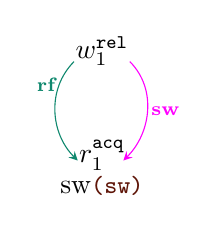
\begin{tikzpicture}[x=1em,y=1em,yscale=-1,xscale=-1]
\tikzstyle{every node}=[font=\normalfont]
\node (w1) {$ w^\rel_1 $};
\node (r1) [below=20pt of w1] {$ r^\acq_1 $};
\node (sw) [below=-5pt of r1] {\hlref{sw}};

\draw [->,>=stealth,color=Magenta] ($ (w1.south east)+(.3,-5pt) $) to[out=135,in=-135] node[midway,right=-2pt,font=\scriptsize] {\textcolor{black}{\lsw}} ($ (r1.south east)+(0.4,-7pt) $);
\draw [->,>=stealth,color=PineGreen] ($ (w1.south west)+(-.3,-5pt) $) to[out=45,in=-45] node[left=-2pt,pos=.25,font=\scriptsize] {\textcolor{black}{\lrf}}($ (r1.south west)+(-0.3,-7pt) $);

\end{tikzpicture}
} &
		\resizebox{0.14\textwidth}{!}{\tikzset{every picture/.style={line width=0.75pt}} %set default line width to 0.75pt        
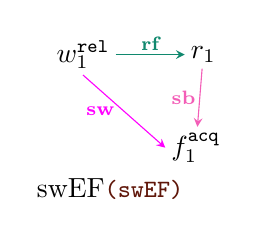
\begin{tikzpicture}[x=1em,y=1em,yscale=-1,xscale=-1]
\tikzstyle{every node}=[font=\normalfont]
\node (w1) [inner sep=2pt] {$ w^\rel_1 $};
\node (r1) [right=25pt of w1,inner sep=2pt] {$ r_1 $};
\node (f1) [below left=21pt and -15pt of r1,inner sep=2pt] {$ f^\acq_1 $};
\node (swef) [below left=0pt and -10pt of f1] {\hlref{swEF}};

`\draw [->,>=stealth,color=Magenta,thin] (w1.south) -- node[midway,left=0pt,font=\scriptsize,color=black] { $\lsw$ } (f1.west);
\draw [->,>=stealth,color=PineGreen,thin] (w1) -- node[midway,above=-2pt,font=\scriptsize,color=black] { $ \lrf $ }  (r1);
\draw [->,>=stealth,color=CarnationPink,thin] (r1) -- node[midway,left=-2pt,font=\scriptsize,color=black] { $\lsb$ } (f1);

\end{tikzpicture}
} &
		\resizebox{0.14\textwidth}{!}{\tikzset{every picture/.style={line width=0.75pt}} %set default line width to 0.75pt        
\begin{tikzpicture}[x=1em,y=1em,yscale=-1,xscale=-1]
\tikzstyle{every node}=[font=\normalfont]
\node [inner sep=2pt] (f1) {$ f^\rel_1 $};
\node (w1) [below left=21pt and -15pt of f1,inner sep=2pt] {$ w_1 $};
\node (r1) [right=25pt of w1,inner sep=2pt] {$ r^\acq_1 $};
\node (swfe) [below right=0pt and -15pt of wr1] {\hlref{sw-dobFE}};

`\draw [->,>=stealth,color=Magenta,thin] (f1.east) -- node[midway,right=0pt,font=\scriptsize,color=black] { $\lsw$ } (r1.north);
\draw [->,>=stealth,color=PineGreen,thin] (w1) -- node[midway,above=-2pt,font=\scriptsize,color=black] { $ \lrf $ } (r1);
\draw [->,>=stealth,color=CarnationPink,thin] (f1) -- node[midway,left=-2pt,font=\scriptsize,color=black] { $\lsb$ } (w1);

\end{tikzpicture}
} &
		\resizebox{0.17\textwidth}{!}{\tikzset{every picture/.style={line width=0.75pt}} %set default line width to 0.75pt        
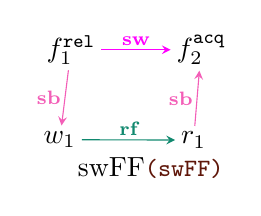
\begin{tikzpicture}[x=1em,y=1em,yscale=-1,xscale=-1]
\tikzstyle{every node}=[font=\normalfont]
\node (f1) [inner sep=2pt] {$ f^\rel_1 $};
\node (f2) [right=25pt of f1,inner sep=2pt] {$ f^\acq_2 $};
\node (w1) [below left=20pt and -15pt of f1,inner sep=2pt] {$ w_1 $};
\node (r1) [below left=20pt and -15pt of f2,inner sep=2pt] {$ r_1 $};
\node (swff) [below right=-2pt and -5pt of w1] {\hlref{swFF}};

`\draw [->,>=stealth,color=Magenta] (f1) -- node[midway,above=-2pt,font=\scriptsize,color=black] { $\lsw$ } (f2);
\draw [->,>=stealth,color=PineGreen] (w1) -- node[midway,above=-2pt,font=\scriptsize,color=black]{\lrf} (r1);
\draw [->,>=stealth,color=CarnationPink] (f1) -- node[midway,left=-2pt,font=\scriptsize,color=black] { $\lsb$ } (w1);
\draw [->,>=stealth,color=CarnationPink] (r1) -- node[midway,left=-2pt,font=\scriptsize,color=black] { $\lsb$ } (f2);

%\draw [->,>=stealth,color=orange] ($ (ew1.south east)+(.5,-5pt) $) to[out=135,in=-135] node[midway,right=-2pt,font=\scriptsize] {mo} ($ (ew2.south east)+(0.4,-5pt) $);
%\draw [->,>=stealth,color=red] ($ (ew1.south west)+(-.3,-5pt) $) to[out=45,in=-45] node[midway,left=-2pt,font=\scriptsize] {c::hb} ($ (ew2.south west)+(-0.3,-5pt) $);


\end{tikzpicture}
} &
		
		\resizebox{0.16\textwidth}{!}{\tikzset{every picture/.style={line width=0.75pt}} %set default line width to 0.75pt        
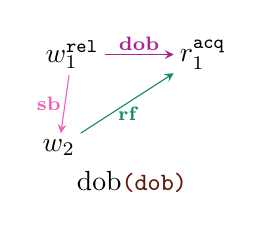
\begin{tikzpicture}[x=1em,y=1em,yscale=-1,xscale=-1]
\tikzstyle{every node}=[font=\normalfont]
\node (w1) [inner sep=2pt] {$ w^\rel_1 $};
\node (r1) [right=25pt of w1,inner sep=2pt] {$ r^\acq_1 $};
\node (w2) [below left=21pt and -15pt of w1,inner sep=2pt] {$ w_2 $};
\node (dob) [below right=0pt and -5pt of w2] {\hlref{dob}};

`\draw [->,>=stealth,color=Mulberry] (w1.east) -- node[midway,above=-2pt,font=\scriptsize,color=black] { $\ldob$ } (r1.west);
\draw [->,>=stealth,color=PineGreen] (w2) -- node[midway,below=-2pt,font=\scriptsize,color=black] { $ \lrf $ }  (r1);
\draw [->,>=stealth,color=CarnationPink] (w1) -- node[midway,left=-2pt,font=\scriptsize,color=black] { $\lsb$ } (w2);

\end{tikzpicture}
} &
		\resizebox{0.17\textwidth}{!}{\tikzset{every picture/.style={line width=0.75pt}} %set default line width to 0.75pt        
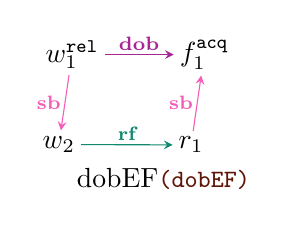
\begin{tikzpicture}[x=1em,y=1em,yscale=-1,xscale=-1]
\tikzstyle{every node}=[font=\normalfont]
\node (w1) [inner sep=2pt] {$ w^\rel_1 $};
\node (f1) [right=25pt of w1,inner sep=2pt] {$ f^\acq_1 $};
\node (w2) [below left=20pt and -15pt of w1,inner sep=2pt] {$ w_2 $};
\node (r1) [below left=20pt and -13pt of f1,inner sep=2pt] {$ r_1 $};
\node (dobEF) [below right=0pt and -5pt of w2] {\hlref{dobEF}};

`\draw [->,>=stealth,color=PineGreen,thin] (w2) -- node[midway,above=-2pt,font=\scriptsize,color=black] { $\lrf$ } (r1);
\draw [->,>=stealth,color=CarnationPink,thin] (w1) -- node[midway,left=-2pt,font=\scriptsize,color=black] { $ \lsb $ } (w2);
\draw [->,>=stealth,color=CarnationPink,thin] (r1) -- node[midway,left=-2pt,font=\scriptsize,color=black] { $\lsb$ } (f1);
\draw [->,>=stealth,color=Mulberry,thin] (w1) -- node[midway,above=-2pt,font=\scriptsize,color=black] { $\ldob$ } (f1);

\end{tikzpicture}
} \\
		\hline
		\multicolumn{4}{c}{(a) \lsw relation} &
		\multicolumn{2}{c}{(b) \ldob relation} \\
	\end{tabular}
	\label{fig:sw}
\end{figure}

\noindent
Formally, $\setSW$ relation is formed using fences as,

$\forall e_1, e_2 \in \events_\tau$ \st $\rf{\tau}{e_1}{e_2}$

if
$e_1 \in \ordwrites{\moge\rel}_\tau$, 
$\exists \mathbb{F}^\acq \in \ordfences{\moge\acq}_{\tau}$ where
$\seqb{\tau}{e_2}{\mathbb{F}^\acq}$ then
$\sw{\tau}{e_1}{\mathbb{F}^\acq}$;

if
$e_2 \in \ordreads{\moge\acq}_\tau$, 
$\exists \mathbb{F}^\rel \in \ordfences{\moge\rel}_{\tau}$ where
$\seqb{\tau}{\mathbb{F}^\rel}{e_1}$ then
$\sw{\tau}{\mathbb{F}^\rel}{e_2}$;

if
$\exists \mathbb{F}^\rel \in \ordfences{\moge\rel}_{\tau}$,
$\mathbb{F}^\acq \in \ordfences{\moge\acq}_{\tau}$ where
$\seqb{\tau}{\mathbb{F}^\rel}{e_1}$,
$\seqb{\tau}{e_2}{\mathbb{F}^\acq}$ 

then
$\sw{\tau}{\mathbb{F}^\rel}{\mathbb{F}^\acq}$.

\noindent
Similarly, $\setDOB$ relation is formed using fences as,

$\forall e_1, e_2 \in \events_\tau$, 
$e_1' \in \ordwrites{\moge\rel}_\tau$ \st $\rf{\tau}{e_1}{e_2}$
and $e_1 \in$ {\em release-sequence}($e_1'$)

if $\exists \mathbb{F}^\acq \in \ordfences{\moge\acq}_{\tau}$ 
where $\seqb{\tau}{e_2}{\mathbb{F}^\acq}$ then
$\dob{\tau}{e_1'}{\mathbb{F}^\acq}$.

\noindent
Further, as is the case with program events,
if $\sw{\tau}{e_1}{e_2}$ or $\dob{\tau}{e_1}{e_2}$ then
events $e_1',e_2'$ \st $\seqb{\tau}{e_1'}{e_1}$ and 
$\seqb{\tau}{e_2}{e_2'}$ are related as $\ithb{\tau}{e_1'}{e_2'}$.

\section{Invalidating buggy sequences with fences} \label{sec:so theory}
Consider a buggy input program $P$.
%
As discussed in Section~\ref{sec:c11}, in a valid trace of $P$ 
(including a buggy trace \aka a counter example), 
the \sc ordered events must form a total order ($\setTO$).
%
Contrarily, if we synthesize \sc ordered fences in the input program 
such that the total order requirement in the buggy trace gets violated 
then we can invalidate the trace and stop the program behavior.
This concept forms the base of our synthesis technique.

We introduce an irreflexive and possibly cyclic relation
on \sc ordered events called \sc-order ($\setSO$).
%
To construct the $\setSO$ order, we introduce the following \lso-rules
(diagrammatically shown in Figure~\ref{fig:so rules}).
The \lso-rules are an interpretation or simply a derivative 
of the \lto-rules, \hlref{toHbMo}, \hlref{toFr} and \hlref{toRf} 
(Section~\ref{sec:c11}).
%formed by direct derivative and dual of the rules .

\begin{figure}[t]
	\begin{tabular}{|c||c|c|c|}
		\multicolumn{1}{c}{base rule} & 
		\multicolumn{3}{c}{extended fence rules} \\\hline
		
		\resizebox{0.24\textwidth}{!}{\tikzset{every picture/.style={line width=0.75pt}} %set default line width to 0.75pt        
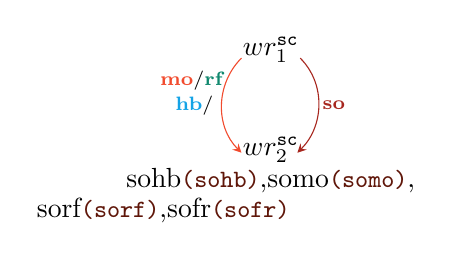
\begin{tikzpicture}[x=1em,y=1em,yscale=-1,xscale=-1]
\tikzstyle{every node}=[font=\normalfont]
\node (wr1) {$ wr^\sc_1 $};
\node (wr2) [below=20pt of wr1] {$ wr^\sc_2 $};
\node (so1) [below=-5pt of wr2] {\hlref{sohb},\hlref{somo},};
\node (so2) [below left=-5pt and -66pt of so1] {\hlref{sorf},\hlref{sofr}};

\draw [->,>=stealth,color=Mahogany,thin] ($ (wr1.south east)+(.3,-5pt) $) to[out=135,in=-135] node[midway,right=-2pt,font=\scriptsize] {\textcolor{black}{\lso}} ($ (wr2.south east)+(0.4,-7pt) $);
\draw [->,>=stealth,color=RedOrange,thin] ($ (wr1.south west)+(-.3,-5pt) $) to[out=45,in=-45] node[left=-2pt,pos=.25,font=\scriptsize] {\textcolor{black}{\lmo/\lrf}} node[left=-0.5pt,pos=.5,font=\scriptsize] {\textcolor{black}{\lhb/\lfr}} ($ (wr2.south west)+(-0.3,-7pt) $);




%\node (nodeB) {$ b: r_1 \assign x  $};
%\node (sigB1) [below left=-3pt and -5pt of nodeB, color=green] {$\sigma_{b11} = $};
%\node (poB1empty) [right=-1pt of sigB1, color=green] {$ $};
%\node (poB1) [draw,fit=(poB1empty), color=orange, thin, inner sep=0pt] {};
%%\node (poB1n1) [right=-3pt of sigB1, color=green] {$ $};
%%\node (poB1) [draw,fit=(poB1n1), color=orange, thin, inner sep=0pt] {};
%\node (B1Val) [right=-3pt of poB1, color=green] {$,0$};
%\node (sigB1State) [fit=(poB1)(B1Val)(sigB1), inner sep=-1pt] {}; 

%\node (sigB2) [right=-3pt of sigB1State, color=green] {$\sigma_{b22} = $};
%\node (poB2N1) [right=6pt of sigB2, circle,fill=black,inner sep=0pt,minimum size=3pt] {};
%\node (poB2a) [left=1pt of poB2N1, inner sep=1pt] {$a$};
%\node (poB2) [draw,fit=(poB2N1)(poB2a), color=orange, thin, inner sep=1pt] {};
%\node (B2Val) [right=-3pt of poB2, color=green] {$,1$};
%\node (sigB2State) [fit=(poB2)(B2Val)(sigB2), inner sep=0pt] {}; 
%
%
%
%%\node (rhoB1) [below =10pt of sigB1State, color=red] {$\rho_{b1}:=0$};
%%\node (rhoB2) [below =10pt of sigB2State, color=red] {$\rho_{b2}:=1$};
%
%
%\node (nodeC) [below =2 of nodeB] {$c: x \assign 2$};
%\node (sigC1) [below left=3pt and -4pt of nodeC, color=green] {$\sigma_{c11} = $};
%\node (poC1N1) [right=6pt of sigC1, circle,fill=black,inner sep=0pt,minimum size=3pt] {};
%\node (poC1c) [left=1pt of poC1N1, inner sep=1pt] {$c$};
%\node (poC1) [draw,fit=(poC1c)(poC1N1), color=orange, thin, inner sep=1pt] {};
%\node (C1Val) [right=-3pt of poC1, color=green] {$,2$};
%\node (sigC1State) [fit=(poC1)(C1Val)(sigC1), inner sep=0pt] {}; 
%
%\node (sigC2) [right=-3pt of sigC1State, color=green] {$\sigma_{c22} = $};
%\node (poC2n1) [above right=0pt and 5pt of sigC2, circle,fill=black,inner sep=0pt,minimum size=3pt] {};
%\node (poC2a) [left=1pt of poC2n1, inner sep=0pt] {$a$};
%\node (poC2n2) [below=9pt of poC2n1, circle,fill=black,inner sep=0pt,minimum size=3pt] {};
%\node (poC2c) [left=1pt of poC2n2, inner sep=0pt] {$c$};
%\draw [color=purple] (poC2n1) -- (poC2n2);
%\node (poC2) [draw,fit=(poC2n1)(poC2a)(poC2n2)(poC2c), color=orange, thin, inner sep=1pt] {};
%\node (C2Val) [right=-3pt of poC2, color=green] {$,2$};
%\node (sigC2State) [fit=(poC2)(C2Val)(sigC2), inner sep=0pt] {}; 
%
%
%
%%\node (rhoC) [below=30pt of nodeC, color=red] {$\rho_{c}=2$};
%
%\node (nodeA) [left =3.5 of nodeB] {$a: x \assign 1$};
%\node (sigA) [below left=-2pt and -25pt of nodeA, color=green] {$\sigma_{a11} = $};
%\node (poAN1) [right=6pt of sigA, circle,fill=black,inner sep=0pt,minimum size=3pt] {};
%\node (poAa) [left=1pt of poAN1, inner sep=1pt] {$a$};
%\node (poA) [draw,fit=(poAN1)(poAa), color=orange, thin, inner sep=1pt] {};
%\node (AVal) [right=-3pt of poA, color=green] {$,1$};
%\node (sigAState) [fit=(poA)(AVal)(sigA), inner sep=-1pt] {}; 
%
%%\node (rhoA) [below=1pt of sigAState, color=red] {$\rho_{a} := 1$};
%
%
%\node (nodeD) [right =5.5 of nodeB] {$ d: r_2 \assign x  $};
%\node (sigD1) [below left=3pt and -5pt of nodeD, color=green] {$\sigma_{d22} = $};
%\node (poD1N1) [right=6pt of sigD1, circle,fill=black,inner sep=0pt,minimum size=3pt] {};
%\node (poD1c) [left=1pt of poD1N1, inner sep=1pt] {$c$};
%\node (poD1) [draw,fit=(poD1c)(poD1N1), color=orange, thin, inner sep=1pt] {};
%\node (D1Val) [right=-3pt of poD1, color=green] {$,2$};
%\node (sigD1State) [fit=(poD1)(D1Val)(sigD1), inner sep=0pt] {}; 
%
%\node (sigD2) [right=-3pt of sigD1State, color=green] {$\sigma_{d33} = $};
%\node (poD2n1) [above right=0pt and 5pt of sigD2, circle,fill=black,inner sep=0pt,minimum size=3pt] {};
%\node (poD2a) [left=1pt of poD2n1, inner sep=0pt] {$a$};
%\node (poD2n2) [below=9pt of poD2n1, circle,fill=black,inner sep=0pt,minimum size=3pt] {};
%\node (poD2c) [left=1pt of poD2n2, inner sep=0pt] {$c$};
%\draw [color=purple] (poD2n1) -- (poD2n2);
%\node (poD2) [draw,fit=(poD2n1)(poD2a)(poD2n2)(poD2c), color=orange, thin, inner sep=1pt] {};
%\node (D2Val) [right=-3pt of poD2, color=green] {$,2$};
%\node (sigD2State) [fit=(poD2)(D2Val)(sigD2), inner sep=0pt] {};  
%
%
%
%\node (nodeE) [below =2 of nodeD] {$e: r_3 \assign x$};
%\node (sigE1) [below left=3pt and -5pt of nodeE, color=green] {$\sigma_{e23} = $};
%\node (poE1N1) [right=6pt of sigE1, circle,fill=black,inner sep=0pt,minimum size=3pt] {};
%\node (poE1c) [left=1pt of poE1N1, inner sep=1pt] {$c$};
%\node (poE1) [draw,fit=(poE1c)(poE1N1), color=orange, thin, inner sep=1pt] {};
%\node (E1Val) [right=-3pt of poE1, color=green] {$,2$};
%\node (sigE1State) [fit=(poE1)(E1Val)(sigE1), inner sep=0pt] {}; 
%
%\node (sigE2) [right=-3pt of sigE1State, color=green] {$\sigma_{e34} = $};
%\node (poE2n1) [above right=0pt and 5pt of sigE2, circle,fill=black,inner sep=0pt,minimum size=3pt] {};
%\node (poE2a) [left=1pt of poE2n1, inner sep=0pt] {$a$};
%\node (poE2n2) [below=9pt of poE2n1, circle,fill=black,inner sep=0pt,minimum size=3pt] {};
%\node (poE2c) [left=1pt of poE2n2, inner sep=0pt] {$c$};
%\draw [color=purple] (poE2n1) -- (poE2n2);
%\node (poE2) [draw,fit=(poE2n1)(poE2a)(poE2n2)(poE2c), color=orange, thin, inner sep=1pt] {};
%\node (E2Val) [right=-3pt of poE2, color=green] {$,2$};
%\node (sigE2State) [fit=(poE2)(E2Val)(sigE2), inner sep=0pt] {}; 
%
%\node (sigE3) [below =9pt of sigE1, color=green] {$\sigma_{e32} = $};
%\node (poE3n1) [above right=0pt and 5pt of sigE3, circle,fill=black,inner sep=0pt,minimum size=3pt] {};
%\node (poE3c) [left=1pt of poE3n1, inner sep=0pt] {$c$};
%\node (poE3n2) [below=9pt of poE3n1, circle,fill=black,inner sep=0pt,minimum size=3pt] {};
%\node (poE3a) [left=1pt of poE3n2, inner sep=0pt] {$a$};
%\draw [color=purple] (poE3n1) -- (poE3n2);
%\node (poE3) [draw,fit=(poE3n1)(poE3a)(poE3n2)(poE3c), color=orange, thin, inner sep=1pt] {};
%\node (E3Val) [right=-3pt of poE3, color=green] {$,1$};
%\node (sigE3State) [fit=(poE3)(E3Val)(sigE3), inner sep=0pt] {};
%
%\node (sigE4) [right =-11pt of sigE3State, color=green] {$\quad \sigma_{e35} = \bot$};
%\node (sigE4State) [fit=(sigE4), inner sep=1pt] {};
%
%
%
%
%%\draw [dashed,->,>=stealth,color=brown,thin] (sigB1State.west) to[out=45,in=-45] (sigC1State.west);
%%\draw [dashed,->,>=stealth,color=brown,thin] (sigB2State.west) to[out=45,in=-45] (sigC2State.west);
%%\draw [dashed,->,>=stealth,color=brown,thin] (sigD1State.west) to[out=45,in=-45] (sigE1State.west);
%%\draw [dashed,->,>=stealth,color=brown,thin] (sigD2State.west) to[out=45,in=-45] (sigE2State.west);
%%\draw [dashed,->,>=stealth,color=brown,thin] (sigD1State.east) to[out=135,in=-135] (sigE3State.east);
%%\draw [dashed,->,>=stealth,color=brown,thin] (sigD2State.east) to[out=135,in=-135] (sigE4State.east);
%%\draw [dashed,->,>=stealth,color=blue,thin] (sigC1State.north east) to[out=-110,in=0] node[midway,left] {rf} (sigD1State.west);
%%\draw [dashed,->,>=stealth,color=blue,thin] (sigC2State.east) to[out=-150,in=0] node[midway,left] {rf} (sigD2State.west);
%
%\draw [dashed,->,>=stealth,color=blue,thin] (sigAState) to[out=165,in=25] node[midway,above] {rf} (sigB2State.south);
%\draw [dashed,->,>=stealth,color=blue,thin] (sigC1State.north east) -- node[midway,above] {rf} (sigD1State.south west);
%\draw [dashed,->,>=stealth,color=blue,thin] (sigC2State.north east) -- node[midway,above] {rf} (sigD2State.south west);
%\draw [dashed,->,>=stealth,color=blue,thin] (sigAState) to[out=105,in=15] node[midway,above] { rf} (sigE3State.west);
%\draw [dashed,->,>=stealth,color=blue,thin] (sigAState) to[out=100,in=20] node[midway,above] {rf} (sigE4State.south);

%\draw [dashed,->,>=stealth,color=blue,thin] (rhoA) -- node[midway,above] {rf} (rhoB2);
%\vspace{-10pt}
\end{tikzpicture}
} &
		\resizebox{0.24\textwidth}{!}{\tikzset{every picture/.style={line width=0.75pt}} %set default line width to 0.75pt        
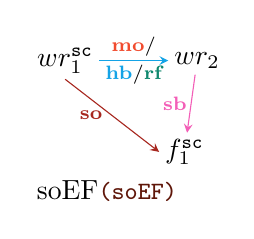
\begin{tikzpicture}[x=1em,y=1em,yscale=-1,xscale=-1]
\tikzstyle{every node}=[font=\normalfont]
\node (wr1) [inner sep=2pt] {$ wr^\sc_1 $};
\node (wr2) [right=25pt of wr1,inner sep=2pt] {$ wr_2 $};
\node (f1) [below left=21pt and -15pt of wr2,inner sep=2pt] {$ f^\sc_1 $};
\node (soef) [below left=0pt and -10pt of f1] {\hlref{soEF}};

`\draw [->,>=stealth,color=Mahogany,thin] (wr1.south) -- node[midway,left=0pt,font=\scriptsize,color=black] { $\lso$ } (f1.west);
\draw [->,>=stealth,color=Cerulean,thin] (wr1) -- node[midway,above=-2pt,font=\scriptsize,color=black] { $ \lmo/ $ } node[midway,below=-2pt,font=\scriptsize,color=black] { $ \lhb/\lrf $ } (wr2);
\draw [->,>=stealth,color=CarnationPink,thin] (wr2) -- node[midway,left=-2pt,font=\scriptsize,color=black] { $\lsb$ } (f1);

\end{tikzpicture}
} &
		\resizebox{0.24\textwidth}{!}{\tikzset{every picture/.style={line width=0.75pt}} %set default line width to 0.75pt        
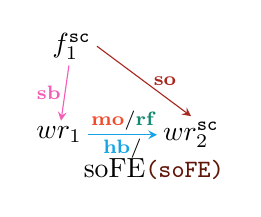
\begin{tikzpicture}[x=1em,y=1em,yscale=-1,xscale=-1]
\tikzstyle{every node}=[font=\normalfont]
\node [inner sep=2pt] (f1) {$ f^\sc_1 $};
\node (wr1) [below left=20pt and -15pt of f1,inner sep=2pt] {$ wr_1 $};
\node (wr2) [right=25pt of wr1,inner sep=2pt] {$ wr^\sc_2 $};
\node (sofe) [below right=0pt and -5pt of wr1] {\hlref{soFE}};

`\draw [->,>=stealth,color=Mahogany] (f1.east) -- node[midway,right=0pt,font=\scriptsize,color=black] { $\lso$ } (wr2.north);
\draw [->,>=stealth,color=Cerulean] (wr1) -- node[midway,above=-2pt,font=\scriptsize,color=black] { $ \lmo/\lrf $ } node[midway,below=-2pt,font=\scriptsize,color=black] { $ \lhb/\lfr $ } (wr2);
\draw [->,>=stealth,color=CarnationPink] (f1) -- node[midway,left=-2pt,font=\scriptsize,color=black] { $\lsb$ } (wr1);

\end{tikzpicture}
} &
		\resizebox{0.24\textwidth}{!}{\tikzset{every picture/.style={line width=0.75pt}} %set default line width to 0.75pt        
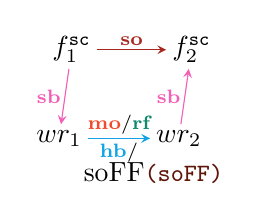
\begin{tikzpicture}[x=1em,y=1em,yscale=-1,xscale=-1]
\tikzstyle{every node}=[font=\normalfont]
\node (f1) [inner sep=2pt] {$ f^\sc_1 $};
\node (f2) [right=25pt of f1,inner sep=2pt] {$ f^\sc_2 $};
\node (wr1) [below left=20pt and -15pt of f1,inner sep=2pt] {$ wr_1 $};
\node (wr2) [below left=20pt and -15pt of f2,inner sep=2pt] {$ wr_2 $};
\node (soff) [below right=0pt and -5pt of wr1] {\hlref{soFF}};

`\draw [->,>=stealth,color=Mahogany] (f1) -- node[midway,above=-2pt,font=\scriptsize,color=black] { $\lso$ } (f2);
\draw [->,>=stealth,color=Cerulean] (wr1) -- node[midway,above=-2pt,font=\scriptsize,color=black]{\lmo/\lrf} node[midway,below=-2pt,font=\scriptsize,color=black]{ $ \lhb/\lfr $ } (wr2);
\draw [->,>=stealth,color=CarnationPink] (f1) -- node[midway,left=-2pt,font=\scriptsize,color=black] { $\lsb$ } (wr1);
\draw [->,>=stealth,color=CarnationPink] (wr2) -- node[midway,left=-2pt,font=\scriptsize,color=black] { $\lsb$ } (f2);

%\draw [->,>=stealth,color=orange] ($ (ew1.south east)+(.5,-5pt) $) to[out=135,in=-135] node[midway,right=-2pt,font=\scriptsize] {mo} ($ (ew2.south east)+(0.4,-5pt) $);
%\draw [->,>=stealth,color=red] ($ (ew1.south west)+(-.3,-5pt) $) to[out=45,in=-45] node[midway,left=-2pt,font=\scriptsize] {c::hb} ($ (ew2.south west)+(-0.3,-5pt) $);


\end{tikzpicture}
} \\
		\hline
%		\hline

%		\resizebox{0.24\textwidth}{!}{\tikzset{every picture/.style={line width=0.75pt}} %set default line width to 0.75pt        
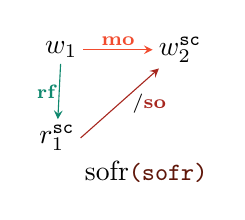
\begin{tikzpicture}[x=1em,y=1em,yscale=-1,xscale=-1]
\tikzstyle{every node}=[font=\normalfont]
\node (w1) [inner sep=2pt] {$ w_1 $};
\node (w2) [right=25pt of w1,inner sep=2pt] {$ w^\sc_2 $};
\node (r1) [below left=20pt and -15pt of w1,inner sep=2pt] {$ r^\sc_1 $};
\node (sofr) [below right=-2pt and -2pt of r1] {\hlref{sofr}};

%\draw [->,>=stealth,color=Mahogany,thin] (er1)+(-7pt, 0) -- node[midway,above=-2pt,font=\scriptsize,color=black] { $\lchb$ } (ew1)+(7pt, 0);
\draw [->,>=stealth,color=RedOrange,thin] (w1) -- node[midway,above=-2pt,font=\scriptsize,color=black] { $\lmo$ } (w2);
\draw [->,>=stealth,color=Mahogany,thin] (r1.east) -- 
node[midway,right=1pt,font=\scriptsize,color=black] { $\lfr/\lso$ } (w2);
\draw [->,>=stealth,color=PineGreen,thin] (w1) -- node[midway,left=-2pt,font=\scriptsize,color=black] { $\lrf$ } (r1);`

\end{tikzpicture}
} &
%		\resizebox{0.24\textwidth}{!}{\tikzset{every picture/.style={line width=0.75pt}} %set default line width to 0.75pt        
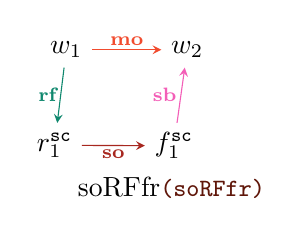
\begin{tikzpicture}[x=1em,y=1em,yscale=-1,xscale=-1]
\tikzstyle{every node}=[font=\normalfont]
\node (w1) {$ w_1 $};
\node (w2) [right=25pt of w1] {$ w_2 $};
\node (r1) [below left=20pt and -15pt of w1] {$ r^\sc_1 $};
\node (f1) [below left=20pt and -15pt of w2] {$ f^\sc_1 $};
\node (sorffr) [below right=0pt and -5pt of r1] {\hlref{soRFfr}};

`\draw [->,>=stealth,color=RedOrange,thin] (w1) -- node[midway,above=-2pt,font=\scriptsize,color=black] { $\lmo$ } (w2);
\draw [->,>=stealth,color=PineGreen,thin] (w1) -- node[midway,left=-2pt,font=\scriptsize,color=black] { $ \lrf $ } (r1);
\draw [->,>=stealth,color=CarnationPink,thin] (f1) -- node[midway,left=-2pt,font=\scriptsize,color=black] { $\lsb$ } (w2);
\draw [->,>=stealth,color=Mahogany,thin] (r1) -- node[midway,below=-2pt,font=\scriptsize,color=black] { $\lso$ } (f1);

\end{tikzpicture}
} &
%		\resizebox{0.24\textwidth}{!}{\tikzset{every picture/.style={line width=0.75pt}} %set default line width to 0.75pt        
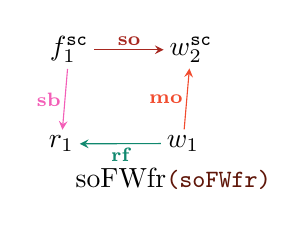
\begin{tikzpicture}[x=1em,y=1em,yscale=-1,xscale=-1]
\tikzstyle{every node}=[font=\normalfont]
\node (f1) [inner sep=2pt] {$ f^\sc_1 $};
\node (w2) [right=25pt of f1,inner sep=2pt] {$ w^\sc_2 $};
\node (r1) [below left=22pt and -13pt of f1,inner sep=2pt] {$ r_1 $};
\node (w1) [below left=22pt and -15pt of w2,inner sep=2pt] {$ w_1 $};
\node (sofwfr) [below right=0pt and -5pt of r1] {\hlref{soFWfr}};

`\draw [->,>=stealth,color=Mahogany,thin] (f1) -- node[midway,above=-2pt,font=\scriptsize,color=black] { $\lso$ } (w2);
\draw [->,>=stealth,color=PineGreen,thin] (w1) -- node[midway,below=-2pt,font=\scriptsize,color=black] { $ \lrf $ } (r1);
\draw [->,>=stealth,color=CarnationPink,thin] (f1) -- node[midway,left=-2pt,font=\scriptsize,color=black] { $\lsb$ } (r1);
\draw [->,>=stealth,color=RedOrange,thin] (w1) -- node[midway,left=-2pt,font=\scriptsize,color=black] { $\lmo$ } (w2);

\end{tikzpicture}
} &
%		\resizebox{0.24\textwidth}{!}{\tikzset{every picture/.style={line width=0.75pt}} %set default line width to 0.75pt        
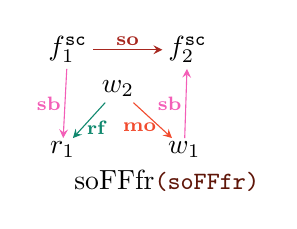
\begin{tikzpicture}[x=1em,y=1em,yscale=-1,xscale=-1]
\tikzstyle{every node}=[font=\normalfont]
\node (f1) [inner sep=2pt] {$ f^\sc_1 $};
\node (f2) [right=25pt of f1,inner sep=2pt] {$ f^\sc_2 $};
\node (r1) [below left=25pt and -13pt of f1, inner sep=1pt] {$ r_1 $};
\node (w1) [below left=25pt and -15pt of f2, inner sep=1pt] {$ w_1 $};
\node (w2) [below right=2pt and 1pt of f1,inner sep=2pt] {$ w_2 $};
\node (sofffr) [below right=0pt and -5pt of r1] {\hlref{soFFfr}};

`\draw [->,>=stealth,color=RedOrange,thin] (w2) -- node[pos=0.7,left=-2pt,font=\scriptsize,color=black] { $\lmo$ } (w1);
\draw [->,>=stealth,color=PineGreen,thin] (w2) -- node[pos=0.7,right=-2pt,font=\scriptsize,color=black] { $ \lrf $ } (r1);
\draw [->,>=stealth,color=CarnationPink,thin] (f1) -- node[midway,left=-2pt,font=\scriptsize,color=black] { $\lsb$ } (r1);
\draw [->,>=stealth,color=CarnationPink,thin] (w1) -- node[midway,left=-2pt,font=\scriptsize,color=black] { $\lsb$ } (f2);
\draw [->,>=stealth,color=Mahogany,thin] (f1) -- node[midway,above=-2pt,font=\scriptsize,color=black] { $\lso$ } (f2);

\end{tikzpicture}
} \\
%		\hline
%		
%		\multicolumn{1}{c||}{} & 
%		\resizebox{0.24\textwidth}{!}{\tikzset{every picture/.style={line width=0.75pt}} %set default line width to 0.75pt        
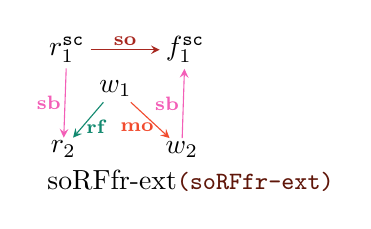
\begin{tikzpicture}[x=1em,y=1em,yscale=-1,xscale=-1]
\tikzstyle{every node}=[font=\normalfont]
\node (r1) [inner sep=2pt] {$ r^\sc_1 $};
\node (f1) [right=25pt of r1,inner sep=2pt] {$ f^\sc_1 $};
\node (r2) [below left=25pt and -13pt of r1, inner sep=1pt] {$ r_2 $};
\node (w2) [below left=25pt and -15pt of f1, inner sep=1pt] {$ w_2 $};
\node (w1) [below right=2pt and 1pt of r1,inner sep=2pt] {$ w_1 $};
\node (sorffrext) [below right=0pt and -15pt of r2] {\hlref{soRFfr-ext}};

`\draw [->,>=stealth,color=RedOrange,thin] (w1) -- node[pos=0.7,left=-2pt,font=\scriptsize,color=black] { $\lmo$ } (w2);
\draw [->,>=stealth,color=PineGreen,thin] (w1) -- node[pos=0.7,right=-2pt,font=\scriptsize,color=black] { $ \lrf $ } (r2);
\draw [->,>=stealth,color=CarnationPink,thin] (r1) -- node[midway,left=-2pt,font=\scriptsize,color=black] { $\lsb$ } (r2);
\draw [->,>=stealth,color=CarnationPink,thin] (w2) -- node[midway,left=-2pt,font=\scriptsize,color=black] { $\lsb$ } (f1);
\draw [->,>=stealth,color=Mahogany,thin] (r1) -- node[midway,above=-2pt,font=\scriptsize,color=black] { $\lso$ } (f1);

\end{tikzpicture}
} &
%		\resizebox{0.24\textwidth}{!}{\tikzset{every picture/.style={line width=0.75pt}} %set default line width to 0.75pt        
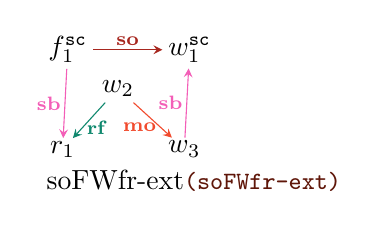
\begin{tikzpicture}[x=1em,y=1em,yscale=-1,xscale=-1]
\tikzstyle{every node}=[font=\normalfont]
\node (f1) [inner sep=2pt] {$ f^\sc_1 $};
\node (wx) [right=25pt of f1,inner sep=2pt] {$ w^\sc_1 $};
\node (r1) [below left=25pt and -13pt of f1, inner sep=1pt] {$ r_1 $};
\node (w2) [below left=25pt and -15pt of wx, inner sep=1pt] {$ w_3 $};
\node (w1) [below right=2pt and 1pt of f1,inner sep=2pt] {$ w_2 $};
\node (sofwfrext) [below right=0pt and -15pt of r1] {\hlref{soFWfr-ext}};

`\draw [->,>=stealth,color=RedOrange,thin] (w1) -- node[pos=0.7,left=-2pt,font=\scriptsize,color=black] { $\lmo$ } (w2);
\draw [->,>=stealth,color=PineGreen,thin] (w1) -- node[pos=0.7,right=-2pt,font=\scriptsize,color=black] { $ \lrf $ } (r1);
\draw [->,>=stealth,color=CarnationPink,thin] (f1) -- node[midway,left=-2pt,font=\scriptsize,color=black] { $\lsb$ } (r1);
\draw [->,>=stealth,color=CarnationPink,thin] (w2) -- node[midway,left=-2pt,font=\scriptsize,color=black] { $\lsb$ } (wx);
\draw [->,>=stealth,color=Mahogany,thin] (f1) -- node[midway,above=-2pt,font=\scriptsize,color=black] { $\lso$ } (wx);

\end{tikzpicture}
} & 
%		\multicolumn{1}{|c}{}\\
%		\cline{2-3}
	\end{tabular}
	\caption{\lso-rules}
	\label{fig:so rules}
\end{figure}

\begin{figure}[t]
	\begin{tabular}{|c||c|c|c|}
		\multicolumn{1}{c}{base rule} & 
		\multicolumn{3}{c}{extended fence rules} \\\hline
		
		\resizebox{0.24\textwidth}{!}{\tikzset{every picture/.style={line width=0.75pt}} %set default line width to 0.75pt        
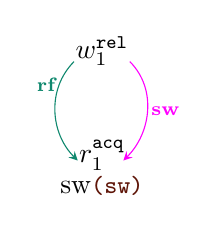
\begin{tikzpicture}[x=1em,y=1em,yscale=-1,xscale=-1]
\tikzstyle{every node}=[font=\normalfont]
\node (w1) {$ w^\rel_1 $};
\node (r1) [below=20pt of w1] {$ r^\acq_1 $};
\node (sw) [below=-5pt of r1] {\hlref{sw}};

\draw [->,>=stealth,color=Magenta] ($ (w1.south east)+(.3,-5pt) $) to[out=135,in=-135] node[midway,right=-2pt,font=\scriptsize] {\textcolor{black}{\lsw}} ($ (r1.south east)+(0.4,-7pt) $);
\draw [->,>=stealth,color=PineGreen] ($ (w1.south west)+(-.3,-5pt) $) to[out=45,in=-45] node[left=-2pt,pos=.25,font=\scriptsize] {\textcolor{black}{\lrf}}($ (r1.south west)+(-0.3,-7pt) $);

\end{tikzpicture}
} &
		\resizebox{0.24\textwidth}{!}{\tikzset{every picture/.style={line width=0.75pt}} %set default line width to 0.75pt        
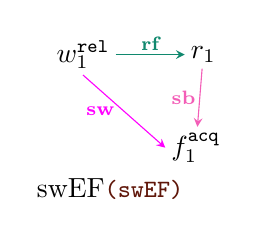
\begin{tikzpicture}[x=1em,y=1em,yscale=-1,xscale=-1]
\tikzstyle{every node}=[font=\normalfont]
\node (w1) [inner sep=2pt] {$ w^\rel_1 $};
\node (r1) [right=25pt of w1,inner sep=2pt] {$ r_1 $};
\node (f1) [below left=21pt and -15pt of r1,inner sep=2pt] {$ f^\acq_1 $};
\node (swef) [below left=0pt and -10pt of f1] {\hlref{swEF}};

`\draw [->,>=stealth,color=Magenta,thin] (w1.south) -- node[midway,left=0pt,font=\scriptsize,color=black] { $\lsw$ } (f1.west);
\draw [->,>=stealth,color=PineGreen,thin] (w1) -- node[midway,above=-2pt,font=\scriptsize,color=black] { $ \lrf $ }  (r1);
\draw [->,>=stealth,color=CarnationPink,thin] (r1) -- node[midway,left=-2pt,font=\scriptsize,color=black] { $\lsb$ } (f1);

\end{tikzpicture}
} &
		\resizebox{0.24\textwidth}{!}{\tikzset{every picture/.style={line width=0.75pt}} %set default line width to 0.75pt        
\begin{tikzpicture}[x=1em,y=1em,yscale=-1,xscale=-1]
\tikzstyle{every node}=[font=\normalfont]
\node [inner sep=2pt] (f1) {$ f^\rel_1 $};
\node (w1) [below left=21pt and -15pt of f1,inner sep=2pt] {$ w_1 $};
\node (r1) [right=25pt of w1,inner sep=2pt] {$ r^\acq_1 $};
\node (swfe) [below right=0pt and -15pt of wr1] {\hlref{sw-dobFE}};

`\draw [->,>=stealth,color=Magenta,thin] (f1.east) -- node[midway,right=0pt,font=\scriptsize,color=black] { $\lsw$ } (r1.north);
\draw [->,>=stealth,color=PineGreen,thin] (w1) -- node[midway,above=-2pt,font=\scriptsize,color=black] { $ \lrf $ } (r1);
\draw [->,>=stealth,color=CarnationPink,thin] (f1) -- node[midway,left=-2pt,font=\scriptsize,color=black] { $\lsb$ } (w1);

\end{tikzpicture}
} &
		\resizebox{0.24\textwidth}{!}{\tikzset{every picture/.style={line width=0.75pt}} %set default line width to 0.75pt        
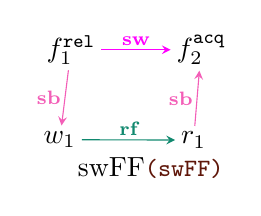
\begin{tikzpicture}[x=1em,y=1em,yscale=-1,xscale=-1]
\tikzstyle{every node}=[font=\normalfont]
\node (f1) [inner sep=2pt] {$ f^\rel_1 $};
\node (f2) [right=25pt of f1,inner sep=2pt] {$ f^\acq_2 $};
\node (w1) [below left=20pt and -15pt of f1,inner sep=2pt] {$ w_1 $};
\node (r1) [below left=20pt and -15pt of f2,inner sep=2pt] {$ r_1 $};
\node (swff) [below right=-2pt and -5pt of w1] {\hlref{swFF}};

`\draw [->,>=stealth,color=Magenta] (f1) -- node[midway,above=-2pt,font=\scriptsize,color=black] { $\lsw$ } (f2);
\draw [->,>=stealth,color=PineGreen] (w1) -- node[midway,above=-2pt,font=\scriptsize,color=black]{\lrf} (r1);
\draw [->,>=stealth,color=CarnationPink] (f1) -- node[midway,left=-2pt,font=\scriptsize,color=black] { $\lsb$ } (w1);
\draw [->,>=stealth,color=CarnationPink] (r1) -- node[midway,left=-2pt,font=\scriptsize,color=black] { $\lsb$ } (f2);

%\draw [->,>=stealth,color=orange] ($ (ew1.south east)+(.5,-5pt) $) to[out=135,in=-135] node[midway,right=-2pt,font=\scriptsize] {mo} ($ (ew2.south east)+(0.4,-5pt) $);
%\draw [->,>=stealth,color=red] ($ (ew1.south west)+(-.3,-5pt) $) to[out=45,in=-45] node[midway,left=-2pt,font=\scriptsize] {c::hb} ($ (ew2.south west)+(-0.3,-5pt) $);


\end{tikzpicture}
} \\
		
		\resizebox{0.24\textwidth}{!}{\tikzset{every picture/.style={line width=0.75pt}} %set default line width to 0.75pt        
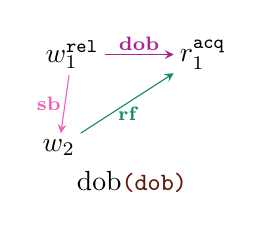
\begin{tikzpicture}[x=1em,y=1em,yscale=-1,xscale=-1]
\tikzstyle{every node}=[font=\normalfont]
\node (w1) [inner sep=2pt] {$ w^\rel_1 $};
\node (r1) [right=25pt of w1,inner sep=2pt] {$ r^\acq_1 $};
\node (w2) [below left=21pt and -15pt of w1,inner sep=2pt] {$ w_2 $};
\node (dob) [below right=0pt and -5pt of w2] {\hlref{dob}};

`\draw [->,>=stealth,color=Mulberry] (w1.east) -- node[midway,above=-2pt,font=\scriptsize,color=black] { $\ldob$ } (r1.west);
\draw [->,>=stealth,color=PineGreen] (w2) -- node[midway,below=-2pt,font=\scriptsize,color=black] { $ \lrf $ }  (r1);
\draw [->,>=stealth,color=CarnationPink] (w1) -- node[midway,left=-2pt,font=\scriptsize,color=black] { $\lsb$ } (w2);

\end{tikzpicture}
} &
		\resizebox{0.24\textwidth}{!}{\tikzset{every picture/.style={line width=0.75pt}} %set default line width to 0.75pt        
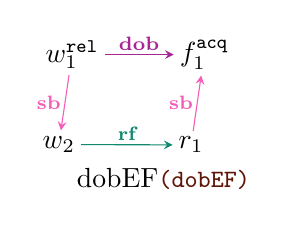
\begin{tikzpicture}[x=1em,y=1em,yscale=-1,xscale=-1]
\tikzstyle{every node}=[font=\normalfont]
\node (w1) [inner sep=2pt] {$ w^\rel_1 $};
\node (f1) [right=25pt of w1,inner sep=2pt] {$ f^\acq_1 $};
\node (w2) [below left=20pt and -15pt of w1,inner sep=2pt] {$ w_2 $};
\node (r1) [below left=20pt and -13pt of f1,inner sep=2pt] {$ r_1 $};
\node (dobEF) [below right=0pt and -5pt of w2] {\hlref{dobEF}};

`\draw [->,>=stealth,color=PineGreen,thin] (w2) -- node[midway,above=-2pt,font=\scriptsize,color=black] { $\lrf$ } (r1);
\draw [->,>=stealth,color=CarnationPink,thin] (w1) -- node[midway,left=-2pt,font=\scriptsize,color=black] { $ \lsb $ } (w2);
\draw [->,>=stealth,color=CarnationPink,thin] (r1) -- node[midway,left=-2pt,font=\scriptsize,color=black] { $\lsb$ } (f1);
\draw [->,>=stealth,color=Mulberry,thin] (w1) -- node[midway,above=-2pt,font=\scriptsize,color=black] { $\ldob$ } (f1);

\end{tikzpicture}
} &&\\
		\hline
		
	\end{tabular}
	\caption{\lsw-rules}
	\label{fig:sw rules}
\end{figure}

\begin{longtable}{|p{0.11\textwidth} p{0.88\textwidth}|}
	\hline
	\multicolumn{2}{|l|}{\bf $\setHB$, $\setMO$, $\setRF$ base rules:}\\
	
	\hl{sohb}, \hl{somo},  & 
	$\forall wr^{\sc}_1, wr^{\sc}_2 \in \ordevents{\sc}_\tau$ if 
	$\hb{\tau}{wr^{\sc}_1}{wr^{\sc}_2}$ $\v$ $\mo{\tau}{wr^{\sc}_1}{wr^{\sc}_2}$
	$\v$ $\rf{\tau}{wr^{\sc}_1}{wr^{\sc}_2}$ then 
	$\so{\tau}{wr^{\sc}_1}{wr^{\sc}_2}$ \\
	\hl{sorf}: & ($\setHB$ order implies $\setSO$) \\
	
%	\hl{somo}: & $\forall w^{\sc}_1, w^{\sc}_2 \in \ordwrites{\sc}_\tau$ if 
%	$\mo{\tau}{w^{\sc}_1}{w^{\sc}_2}$
%	then $\so{\tau}{w^{\sc}_1}{w^{\sc}_2}$ \\
%	& ($\setMO$ order implies $\setSO$) \\
%	
%	\hl{sorf}: & $\forall w^{\sc}_1 \in \ordwrites{sc}_\tau$, $r^{\sc}_1 \in 
%	\ordreads{\sc}_\tau$ if $\rf{\tau}{w^{\sc}_1}{r^{\sc}_1}$ then 
%	$\so{\tau}{w^{\sc}_1}{r^{\sc}_1}$ \\
%	& ($\setRF$ order implies $\setSO$) \\
	& \\
	
	\multicolumn{2}{|l|}{\bf $\setHB$, $\setMO$, $\setRF$ rules extended
		for fences:} \\
	
	\hl{soEF}: & $\forall wr^\sc_1 \in \ordevents{\sc}_\tau$, $f^\sc_1 \in
	\ordfences{\sc}_\tau$ if $\exists wr_2 \in \events_\tau$ \st 
	($\mo{\tau}{wr^\sc_1}{wr_2}$ $\v$ $\hb{\tau}{wr^\sc_1}{wr_2}$
	$\v$ $\rf{\tau}{wr^\sc_1}{wr_2}$) $\^$ $\seqb{\tau}{wr_2}{f^\sc_1}$ 
	then $\so{\tau}{wr^\sc_1}{f^\sc_1}$ \\
	& ($\setHB$ between \sc event-fence implies $\setSO$) \\
	
	\hl{soFE}: & $\forall f^\sc_1 \in \ordfences{\sc}_\tau$, $wr^\sc_2 \in
	\ordevents{\sc}_\tau$ if $\exists wr_1 \in \events_\tau$ \st 
	($\mo{\tau}{wr_1}{wr^\sc_2}$ $\v$ $\hb{\tau}{wr_1}{wr^\sc_2}$
	$\v$ $\rf{\tau}{wr_1}{wr^\sc_2}$) $\^$ $\seqb{\tau}{f^\sc_1}{wr_1}$ 
	then $\so{\tau}{f^\sc_1}{wr^\sc_2}$ \\
	& ($\setHB$ between fence-\sc event implies $\setSO$) \\
	
	\hl{soFF}: & $\forall f^{\sc}_1, f^{\sc}_2 \in \ordfences{\sc}_\tau$, 
	if $\exists wr_1, wr_2 \in \events_\tau$ \st 
	($\mo{\tau}{wr_1}{wr_2}$ $\v$ $\hb{\tau}{wr_1}{wr_2}$
	$\v$ $\rf{\tau}{wr_1}{wr_2}$) $\^$
	($\seqb{\tau}{f^{\sc}_1}{wr_1}$, $\seqb{\tau}{wr_2}{f^{\sc}_2}$) 
	then $\so{\tau}{f^{\sc}_1}{f^{\sc}_2}$ \\
	& ($\setHB$ between \sc fence-fences implies $\setSO$) \\
	\hline
\end{longtable}
	
\begin{longtable}{|p{0.13\textwidth} p{0.86\textwidth}|}
	\hline
	\multicolumn{2}{|l|}{\bf $\setFR$ base rule:}\\
	
	\hl{sofr}: & $\forall r^\sc_1 \in \ordreads{\sc}_\tau$, $w^\sc_1 \in
	\ordwrites{\sc}_\tau$ if $\fr{\tau}{r^\sc_1}{w^sc_1}$ then 
	$\so{\tau}{r^{\sc}_1}{w^{\sc}_1}$ \\
	& ($\setFR$ order implies $\setSO$) \\
	
	& \\
	
	\multicolumn{2}{|l|}{\bf $\setFR$ rules extended for fences:}\\
	
	\hl{soRFfr}: & $\forall f^\sc_1 \in \ordfences{\sc}_\tau$, $r^\sc_1 \in
	\ordreads{\sc}_\tau$ if $\exists w_1, w_2 \in \writes_\tau$ \st
	$\seqb{\tau}{w_2}{f^\sc_1}$, $\mo{\tau}{w_1}{w_2}$ and
	$\rf{\tau}{w_1}{r^\sc_1}$ then $\so{\tau}{r^\sc_1}{f^\sc_1}$ \\
	& ($\setFR$ though \sc read-fence synchronization implies $\setSO$) \\
	
	\hl{soRFfr-ext}: & \tab $\forall r^\sc_1 \in \ordreads{\sc}_\tau$, $f^\sc_1 
	\in \ordfences{\sc}_\tau$ if $\exists w_1,w_2 \in \writes_\tau$, $r_2 \in
	\reads_\tau$ \st $\seqb{\tau}{r^\sc_1}{r_2}$, $\seqb{\tau}{w_2}{f^\sc_1}$,
	$\mo{\tau}{w_1}{w_2}$ and $\rf{\tau}{w_1}{r_2}$ then 
	$\so{\tau}{r^\sc_1}{f^\sc_1}$ \\
	& ($\setFR$ though \sc read-fence synchronization via $\setSB$ implies 
	$\setSO$) \\
	
	\hl{soFWfr}: & $\forall f^{\sc}_1 \in \ordfences{\sc}_\tau$, $w^{\sc}_1 \in 
	\ordwrites{\sc}_\tau$ if $\exists w_2 \in \writes_\tau$, $r_1 \in 
	\reads_\tau$ \st $\seqb{\tau}{f^{\sc}_1}{r_1}$, $\mo{\tau}{w_2}{w^{\sc}_1}$ 
	and $\rf{\tau}{w_2}{r_1}$ then $\so{\tau}{f^{\sc}_1}{w^{\sc}_1}$ \\
	& ($\setFR$ though \sc write-fence synchronization implies $\setSO$) \\
	
	\hl{soFWfr-ext}: & \tab $\forall f^{\sc}_1 \in \ordfences{\sc}_\tau$, 
	$w^{\sc}_1 \in \ordwrites{\sc}_\tau$ if $\exists w_2, w_3 \in \writes_\tau$, 
	$r_1 \in \reads_\tau$ \st $\seqb{\tau}{f^{\sc}_1}{r_1}$, 
	$\seqb{\tau}{w_3}{w^\sc_1}$, $\mo{\tau}{w_2}{w_3}$ and $\rf{\tau}{w_2}{r_1}$ 
	then $\so{\tau}{f^\sc_1}{w^\sc_1}$ \\
	& ($\setFR$ though \sc write-fence synchronization via $\setSB$ implies 
	$\setSO$) \\
	
	\hl{soFFfr}: & $\forall f^\sc_1, f^\sc_2 \in \ordfences{\sc}_\tau$
	if $\exists$ $w_1, w_2 \in \ordwrites{\sc}_\tau$, $r_1 \in
	\ordreads{\sc}_\tau$ \st $\seqb{\tau}{f^\sc_1}{r_1}$, 
	$\seqb{\tau}{w_1}{f^\sc_2}$, $\mo{\tau}{w_2}{w_1}$ and
	$\rf{\tau}{w_2}{r_1}$ then $\so{\tau}{f^\sc_1}{f^\sc_2}$ \\
	& ($\setFR$ though \sc fence-fence synchronization implies $\setSO$) \\
	\hline
\end{longtable}


%\begin{itemize}[label=soFFnrf,align=left,leftmargin=*]
%	\item [\hl{sohb}:] $\forall wr^{\sc}_1, wr^{\sc}_2 \in \ordevents{\sc}_\tau$ if 
%			$\hb{\tau}{wr^{\sc}_1}{wr^{\sc}_2}$ then 
%			$\so{\tau}{wr^{\sc}_1}{wr^{\sc}_2}$ \newline
%			($\setHB$ order implies $\setSO$)
%	
%	\item [\hl{somo}:] $\forall w^{\sc}_1, w^{\sc}_2 \in \ordwrites{\sc}_\tau$ if 
%			$\mo{\tau}{w^{\sc}_1}{w^{\sc}_2}$
%			then $\so{\tau}{w^{\sc}_1}{w^{\sc}_2}$ \newline
%			($\setMO$ order implies $\setSO$)
%			
%	\item [\hl{sorf}:] $\forall w^{\sc}_1 \in \ordwrites{sc}_\tau$, $r^{\sc}_1 \in 
%			\ordreads{\sc}_\tau$ if $\rf{\tau}{w^{\sc}_1}{r^{\sc}_1}$ then 
%			$\so{\tau}{w^{\sc}_1}{r^{\sc}_1}$ \newline
%			($\setRF$ order implies $\setSO$)
%			
%	\item [\hl{soEF}:] $\forall wr^\sc_1 \in \ordevents{\sc}_\tau$, $f^\sc_1 \in
%			\ordfences{\sc}_\tau$ if $\exists wr_2 \in \events_\tau$ \st 
%			($\mo{\tau}{wr^\sc_1}{wr_2}$ $\v$ $\hb{\tau}{wr^\sc_1}{wr_2}$
%			$\v$ $\rf{\tau}{wr^\sc_1}{wr_2}$) $\^$ $\seqb{\tau}{wr_2}{f^\sc_1}$ 
%			then $\so{\tau}{wr^\sc_1}{f^\sc_1}$\newline
%			($\setHB$ between \sc event-fence implies $\setSO$)
%			
%	\item [\hl{soFE}:] $\forall f^\sc_1 \in \ordfences{\sc}_\tau$, $wr^\sc_2 \in
%			\ordevents{\sc}_\tau$ if $\exists wr_1 \in \events_\tau$ \st 
%			($\mo{\tau}{wr_1}{wr^\sc_2}$ $\v$ $\hb{\tau}{wr_1}{wr^\sc_2}$
%			$\v$ $\rf{\tau}{wr_1}{wr^\sc_2}$) $\^$ $\seqb{\tau}{f^\sc_1}{wr_1}$ 
%			then $\so{\tau}{f^\sc_1}{wr^\sc_2}$\newline
%			($\setHB$ between fence-\sc event implies $\setSO$)
%			
%	\item [\hl{soFF}:]  $\forall f^{\sc}_1, f^{\sc}_2 \in \ordfences{\sc}_\tau$, 
%			if $\exists wr_1, wr_2 \in \events_\tau$ \st 
%			($\mo{\tau}{wr_1}{wr_2}$ $\v$ $\hb{\tau}{wr_1}{wr_2}$
%			$\v$ $\rf{\tau}{wr_1}{wr_2}$) $\^$
%			($\seqb{\tau}{f^{\sc}_1}{wr_1}$, $\seqb{\tau}{wr_2}{f^{\sc}_2}$) 
%			then $\so{\tau}{f^{\sc}_1}{f^{\sc}_2}$ \newline
%			($\setHB$ between \sc fence-fences implies $\setSO$)
%			
%	\item [\hl{sofr}:] $\forall r^\sc_1 \in \ordreads{\sc}_\tau$, $w^\sc_1 \in
%			\ordwrites{\sc}_\tau$ if $\fr{\tau}{r^\sc_1}{w^sc_1}$ then 
%			$\so{\tau}{r^{\sc}_1}{w^{\sc}_1}$ 
%			\newline
%			($\setFR$ order implies $\setSO$)
%			
%	\item [\hl{soFWfr}:] $\forall f^{\sc}_1 \in \ordfences{\sc}_\tau$, $w^{\sc}_1 \in 
%			\ordwrites{\sc}_\tau$ if $\exists w_2 \in \writes_\tau$, $r_1 \in 
%			\reads_\tau$ \st $\seqb{\tau}{f^{\sc}_1}{r_1}$, $\mo{\tau}{w_2}{w^{\sc}_1}$ 
%			and $\rf{\tau}{w_2}{r_1}$ then $\so{\tau}{f^{\sc}_1}{w^{\sc}_1}$ \newline
%			($\setFR$ though \sc write-fence synchronization implies $\setSO$)
%			
%	\item [\hl{soRFfr}:] $\forall f^\sc_1 \in \ordfences{\sc}_\tau$, $r^\sc_1 \in
%			\ordreads{\sc}_\tau$ if $\exists w_1, w_2 \in \writes_\tau$ \st
%			$\seqb{\tau}{w_2}{f^\sc_1}$, $\mo{\tau}{w_1}{w_2}$ and
%			$\rf{\tau}{w_1}{r^\sc_1}$ then $\so{\tau}{r^\sc_1}{f^\sc_1}$\newline
%			($\setFR$ though \sc read-fence synchronization implies $\setSO$)
%			
%	\item [\hl{soFFfr}:] $\forall f^\sc_1, f^\sc_2 \in \ordfences{\sc}_\tau$
%			if $\exists$ $w_1, w_2 \in \ordwrites{\sc}_\tau$, $r_1 \in
%			\ordreads{\sc}_\tau$ \st $\seqb{\tau}{f^\sc_1}{r_1}$, 
%			$\seqb{\tau}{w_1}{f^\sc_2}$, $\mo{\tau}{w_2}{w_1}$ and
%			$\rf{\tau}{w_2}{r_1}$ then $\so{\tau}{f^\sc_1}{f^\sc_2}$\newline
%			($\setFR$ though \sc fence-fence synchronization implies $\setSO$)
%\end{itemize}

Consider a \cc trace $\tau$ and a transformation
$\inv{\tau}$ of $\tau$ \st $\events_{\inv{\tau}}$ = $\events_\tau$
$\union$ set of synthesized fences, then;
%
\begin{theorem}
	$\to{\tau}{}{}$ $\subseteq$ (transitive closure of $\so{\inv{\tau}}{}{}$);
	however, if $\exists$ $\to{\imm{\tau}}{}{}$ then $\to{\imm{\tau}}{}{}$ = 
	(transitive closure of $\so{\inv{\tau}}{}{}$)
\end{theorem}
%
A cyclic $\so{\inv{\tau}}{}{}$ implies that there does not exist a 
total order on \sc ordered events of $\inv{\tau}$. The trace $\inv{\tau}$, 
then, is not a valid \cc trace and the buggy trace $\tau$ 
has been invalidated.
%
Thus, the aim of this work is to synthesis fences in the input program $P$
at appropriate locations and force a cyclic $\setSO$ order in the \sc 
ordered events of a buggy trace $\tau$ of $P$ and invalidating the trace 
for the transformed program $\fx{P}$.

\section{Methodology} \label{sec:methodology}
\section{Implementation Details} \label{sec:implementation}
\section{Results} \label{sec:results}
\section{Related Work} \label{sec:related}
\section{Conclusion} \label{sec:conclusion}

%\bibliographystyle{unsrtnat}
\bibliography{References.bib}


\end{document}
